
\documentclass{article}

%%%%%%%%%%%%%%%%%%%%%%%%%%%%%%%%%%%%%%%%%
% Lachaise Assignment
% Structure Specification File
% Version 1.0 (26/6/2018)
%
% This template originates from:
% http://www.LaTeXTemplates.com
%
% Authors:
% Marion Lachaise & François Févotte
% Vel (vel@LaTeXTemplates.com)
%
% License:
% CC BY-NC-SA 3.0 (http://creativecommons.org/licenses/by-nc-sa/3.0/)
% 
%%%%%%%%%%%%%%%%%%%%%%%%%%%%%%%%%%%%%%%%%

%----------------------------------------------------------------------------------------
%	PACKAGES AND OTHER DOCUMENT CONFIGURATIONS
%----------------------------------------------------------------------------------------
\usepackage[table]{xcolor}
\usepackage{amsmath,amsfonts,stmaryrd,amssymb} % Math packages

\usepackage{enumerate} % Custom item numbers for enumerations

\usepackage{enumitem}

\usepackage[ruled]{algorithm2e} % Algorithms

\usepackage[framemethod=tikz]{mdframed} % Allows defining custom boxed/framed environments

\usepackage{listings} % File listings, with syntax highlighting
\lstset{
	basicstyle=\ttfamily, % Typeset listings in monospace font
}

\usepackage{flafter}

\usepackage{longtable}

\usepackage[utf8]{inputenc}
\usepackage{enumitem, amsfonts, tikz, indentfirst, amssymb, float, amsmath, graphicx, multicol, multirow}
\usepackage[margin=1in]{geometry}
\usepackage{geometry}
\usepackage{booktabs, longtable, lscape, threeparttable}
%----------------------------------------------------------------------------------------
%	DOCUMENT MARGINS
%----------------------------------------------------------------------------------------

\usepackage{geometry} % Required for adjusting page dimensions and margins

\geometry{
	paper=a4paper, % Paper size, change to letterpaper for US letter size
	top=2cm, % Top margin
	bottom=2cm, % Bottom margin
	left=2cm, % Left margin
	right=2cm, % Right margin
	headheight=12pt, % Header height
	footskip=1.5cm, % Space from the bottom margin to the baseline of the footer
	headsep=1cm, % Space from the top margin to the baseline of the header
	%showframe, % Uncomment to show how the type block is set on the page
}


%----------------------------------------------------------------------------------------
%	FONTS
%----------------------------------------------------------------------------------------

\usepackage[utf8]{inputenc} % Required for inputting international characters
\usepackage[T1]{fontenc} % Output font encoding for international characters

\usepackage{XCharter} % Use the XCharter fonts

%----------------------------------------------------------------------------------------
%	COMMAND LINE ENVIRONMENT
%----------------------------------------------------------------------------------------

% Usage:
% \begin{commandline}
%	\begin{verbatim}
%		$ ls
%		
%		Applications	Desktop	...
%	\end{verbatim}
% \end{commandline}

\mdfdefinestyle{commandline}{
	leftmargin=10pt,
	rightmargin=10pt,
	innerleftmargin=15pt,
	middlelinecolor=black!50!white,
	middlelinewidth=2pt,
	frametitlerule=false,
	backgroundcolor=black!5!white,
	frametitle={Command Line},
	frametitlefont={\normalfont\sffamily\color{white}\hspace{-1em}},
	frametitlebackgroundcolor=black!50!white,
	nobreak,
}

% Define a custom environment for command-line snapshots
\newenvironment{commandline}{
	\medskip
	\begin{mdframed}[style=commandline]
}{
	\end{mdframed}
	\medskip
}

%----------------------------------------------------------------------------------------
%	FILE CONTENTS ENVIRONMENT
%----------------------------------------------------------------------------------------

% Usage:
% \begin{file}[optional filename, defaults to "File"]
%	File contents, for example, with a listings environment
% \end{file}

\mdfdefinestyle{file}{
	innertopmargin=0.8 \baselineskip,
	innerbottommargin=0.8\baselineskip,
	topline=false, bottomline=false,
	leftline=false, rightline=false,
	leftmargin=2cm,
	rightmargin=2cm,
	singleextra={%
		\draw[fill=black!10!white](P)++(0,-1.2em)rectangle(P-|O);
		\node[anchor=north west]
		at(P-|O){\ttfamily\mdfilename};
		%
		\def\l{3em}
		\draw(O-|P)++(-\l,0)--++(\l,\l)--(P)--(P-|O)--(O)--cycle;
		\draw(O-|P)++(-\l,0)--++(0,\l)--++(\l,0);
	},
	nobreak,
}

% Define a custom environment for file contents
\newenvironment{file}[1][File]{ % Set the default filename to "File"
	\medskip
	\newcommand{\mdfilename}{#1}
	\begin{mdframed}[style=file]
}{
	\end{mdframed}
	\medskip
}

%----------------------------------------------------------------------------------------
%	NUMBERED QUESTIONS ENVIRONMENT
%----------------------------------------------------------------------------------------

% Usage:
% \begin{question}[optional title]
%	Question contents
% \end{question}

\mdfdefinestyle{question}{
	innertopmargin=0.8\baselineskip,
	innerbottommargin=0.8\baselineskip,
	roundcorner=5pt,
	nobreak,
	singleextra={%
		\draw(P-|O)node[xshift=1em,anchor=west,fill=white,draw,rounded corners=5pt]{%
		Question \theQuestion\questionTitle};
	},
}

\newcounter{Question} % Stores the current question number that gets iterated with each new question

% Define a custom environment for numbered questions
\newenvironment{question}[1][\unskip]{
	\bigskip
	\stepcounter{Question}
	\newcommand{\questionTitle}{~#1}
	\begin{mdframed}[style=question]
}{
	\end{mdframed}
	\medskip
}

%----------------------------------------------------------------------------------------
%	WARNING TEXT ENVIRONMENT
%----------------------------------------------------------------------------------------

% Usage:
% \begin{warn}[optional title, defaults to "Warning:"]
%	Contents
% \end{warn}

\mdfdefinestyle{warning}{
	topline=false, bottomline=false,
	leftline=false, rightline=false,
	nobreak,
	singleextra={%
		\draw(P-|O)++(-0.5em,0)node(tmp1){};
		\draw(P-|O)++(0.5em,0)node(tmp2){};
		\fill[black,rotate around={45:(P-|O)}](tmp1)rectangle(tmp2);
		\node at(P-|O){\color{white}\scriptsize\bf !};
		\draw[very thick](P-|O)++(0,-1em)--(O);%--(O-|P);
	}
}

% Define a custom environment for warning text
\newenvironment{warn}[1][Warning:]{ % Set the default warning to "Warning:"
	\medskip
	\begin{mdframed}[style=warning]
		\noindent{\textbf{#1}}
}{
	\end{mdframed}
}

%----------------------------------------------------------------------------------------
%	INFORMATION ENVIRONMENT
%----------------------------------------------------------------------------------------

% Usage:
% \begin{info}[optional title, defaults to "Info:"]
% 	contents
% 	\end{info}

\mdfdefinestyle{info}{%
	topline=false, bottomline=false,
	leftline=false, rightline=false,
	nobreak,
	singleextra={%
		\fill[black](P-|O)circle[radius=0.4em];
		\node at(P-|O){\color{white}\scriptsize\bf i};
		\draw[very thick](P-|O)++(0,-0.8em)--(O);%--(O-|P);
	}
}

% Define a custom environment for information
\newenvironment{info}[1][Info:]{ % Set the default title to "Info:"
	\medskip
	\begin{mdframed}[style=info]
		\noindent{\textbf{#1}}
}{
	\end{mdframed}
}
 % Include the file specifying the document structure and custom commands
\usepackage{longtable}

%----------------------------------------------------------------------------------------
%	ASSIGNMENT INFORMATION
%----------------------------------------------------------------------------------------

\title{The Link Between Marijuana Legalization and Opioid Overdoses} % Title of the assignment

\author{Shawn Leavor, Colin McNally, Jacob Bulzak} % Author name and email address

%----------------------------------------------------------------------------------------

\begin{document}

\maketitle % Print the title


%----------------------------------------------------------------------------------------
%	Introduction
%----------------------------------------------------------------------------------------

\section*{Abstract} % Unnumbered section

Our goal was to determine if there was a link between opioid deaths and availability of marijuana. To do this, we studied opioid deaths by state from 1999-2020 and did a difference-in-differenes study where the treatment was legalization of marijuana. From 2012 to 2020, 14 states legalized marijuana for recreational use, so we used these states to determine how deaths from opioids changes when a state legalizes marijuana. We find that 5-years after legalizing marijuana, states with legal marijuana see a decrease in opioid deaths relative to those where it is still illegal. 

\section*{Introduction} % Unnumbered section

We are interested in estimating the causal effect of access to marijuana on opioid deaths. The parameter we care about is the average treated on the treated of marijuana legalization on opioid deaths. We believe that marijuana could be a substitute for opioids in use for pain addiction, so we expect that the legalization of marijuana recreationally and easier access to this alternative will cause a reduction in opioid deaths.

The results of this study can enable policy changes that can help lower opioid deaths across the United States, one of the biggest problems that the country is tackling. Other laws, such as limiting prescriptions of opioids can lead to people seeking illegal substitutes, such as heroin. Legalizing marijuana could be an effective policy to combat the growing opioid epidemic. 

%----------------------------------------------------------------------------------------
%	Background and Economic Theory
%----------------------------------------------------------------------------------------

\section*{Background} % Numbered section

Since 2012, 14 states have made recreational use of marijuana legal. Over that same time period, we've seen the death rate of opioids explode, as shown in table 3. With the rise of the opioid crisis, due to many reasons, including prescription of opioids for pain management, people want to find an alternative for opioids. There is some literature that shows that marijuana can be a substitute for pain management, so we examine if there is a linkk between the two and if marijuana is used as a substitute. 

We use legalization of marijuana as a random assignment of ability to use marijuana over opiates. There's no difference between states, except that more liberal states may be more likely to legalize marijuana. We assume that treatment is a random assignment of freedom to use marijuana for opioid users. 

\begin{table} \centering
\caption{Year Marijuana Was Legalized Recreationally}
\label{}
\begin{tabular}[t]{l|r}
\hline
State & Treatment Year\\
\hline
Alaska & 2014\\
\hline
Arizona & 2020\\
\hline
California & 2016\\
\hline
Colorado & 2012\\
\hline
Illinois & 2019\\
\hline
Maine & 2016\\
\hline
Massachusetts & 2016\\
\hline
Michigan & 2018\\
\hline
Montana & 2020\\
\hline
Nevada & 2016\\
\hline
New Jersey & 2020\\
\hline
Oregon & 2014\\
\hline
Vermont & 2018\\
\hline
Washington & 2012\\
\hline
\end{tabular}
\end{table}


%----------------------------------------------------------------------------------------
%	Data
%----------------------------------------------------------------------------------------

\section*{Data} % Numbered section

Data comes from the CDC WONDER system which has data for underlying death cause from 1999 until 2020. Because of this data limitation, we ignore states that legalized marijuana after 2020 and the District of Columbia. Opioid overdose deaths are identified using underlying cause-of-death codes X40–X44, X60–X64, X85, and Y10–Y14. All data comes from the CDC and provides the death rate per 100,000 citizens from opioids for each year for each state. The data also includes the population of each state and total deaths from opioids. 

The below tables show which states have the highest average rate of opioid deaths over the data period and also how the average death rate from opioids changes from year to year. We see that states like West Virginia and New Mexico have a high rate of opioid death, while the less densely populated states of North Dakokta and South Dakota have less. We can also see that the average death rate each year steadily rises and quintupled over the study period. 

\begin{table}\centering
\caption{Mean Opioid Deaths per State from 1999 to 2020}
\label{}
\begin{tabular}[t]{l|r}
\hline
State & Mean Death Rate\\
\hline
Alabama & 11.016523\\
\hline
Alaska & 14.470724\\
\hline
Arizona & 16.903674\\
\hline
Arkansas & 10.787611\\
\hline
California & 10.816570\\
\hline
Colorado & 14.608636\\
\hline
Connecticut & 16.326355\\
\hline
Delaware & 18.629955\\
\hline
Florida & 15.913815\\
\hline
Georgia & 10.161905\\
\hline
Hawaii & 10.650873\\
\hline
Idaho & 10.583673\\
\hline
Illinois & 12.692079\\
\hline
Indiana & 14.742777\\
\hline
Iowa & 7.102904\\
\hline
Kansas & 9.499878\\
\hline
Kentucky & 21.053527\\
\hline
Louisiana & 16.042985\\
\hline
Maine & 15.496395\\
\hline
Maryland & 19.348076\\
\hline
Massachusetts & 17.563764\\
\hline
Michigan & 14.724472\\
\hline
Minnesota & 8.237864\\
\hline
Mississippi & 9.945878\\
\hline
Missouri & 15.143731\\
\hline
Montana & 11.169932\\
\hline
Nebraska & 5.741136\\
\hline
Nevada & 19.320376\\
\hline
New Hampshire & 17.168707\\
\hline
New Jersey & 14.313014\\
\hline
New Mexico & 22.240670\\
\hline
New York & 10.733684\\
\hline
North Carolina & 13.665396\\
\hline
North Dakota & 5.198840\\
\hline
Ohio & 19.290818\\
\hline
Oklahoma & 15.716280\\
\hline
Oregon & 11.792944\\
\hline
Pennsylvania & 19.639422\\
\hline
Rhode Island & 19.014600\\
\hline
South Carolina & 13.456070\\
\hline
South Dakota & 5.784089\\
\hline
Tennessee & 17.897485\\
\hline
Texas & 9.033012\\
\hline
Utah & 17.086345\\
\hline
Vermont & 13.268174\\
\hline
Virginia & 10.816864\\
\hline
Washington & 13.914318\\
\hline
West Virginia & 28.376235\\
\hline
Wisconsin & 12.377786\\
\hline
Wyoming & 11.644840\\
\hline
\end{tabular}
\end{table}

\begin{table}\centering
\caption{Average Death Rate by Year}
\label{}
\begin{tabular}[t]{r|r}
\hline
Year & Mean Death Rate\\
\hline
1999 & 5.737328\\
\hline
2000 & 6.202161\\
\hline
2001 & 7.111196\\
\hline
2002 & 8.295035\\
\hline
2003 & 9.219804\\
\hline
2004 & 9.629441\\
\hline
2005 & 10.295837\\
\hline
2006 & 11.750586\\
\hline
2007 & 12.316517\\
\hline
2008 & 12.669908\\
\hline
2009 & 12.517710\\
\hline
2010 & 12.929883\\
\hline
2011 & 14.068499\\
\hline
2012 & 13.939109\\
\hline
2013 & 14.724975\\
\hline
2014 & 15.842746\\
\hline
2015 & 17.447247\\
\hline
2016 & 20.412369\\
\hline
2017 & 21.994138\\
\hline
2018 & 21.193078\\
\hline
2019 & 22.111916\\
\hline
2020 & 28.085816\\
\hline
\end{tabular}
\end{table}

%----------------------------------------------------------------------------------------
%	Empirical Models
%----------------------------------------------------------------------------------------

\section*{Methodology} % Numbered section

We use our state and year-level data to perform a difference in difference study and examine a causal effect between legalizing marijuana and opioid death rate. The only control we add in this study is for state population each year. 

Our Paper uses the Callaway and Sant'anna Difference in Differences Estimator which uses the following formula to estimate average treatment of the treated:

$$ATT(g,t)=E[(  \frac{G_g}{ E[G_g]} - \frac{ \frac{ \hat{p} (X)C}{1- \hat{p} (X)}}{E [\frac{\hat{p} (X) C } {1 - \hat{p} (X)}]}) (Y_t - Y_{g-1})]$$

\section*{Results}

We find a significant effect after 5 years of legalizing the recreational use of marijuana. The figure below shows our findings. Most states seem to have a comparable difference in opioid deaths leading up to treatment and even for 3 to 4 years afterwards. However, after the 5th year, we see a significant decrease in opioid deaths for our treated states compared to our untreated states and this holds for the rest of the treatment period. 


\begin{figure}
    \begin{center}
        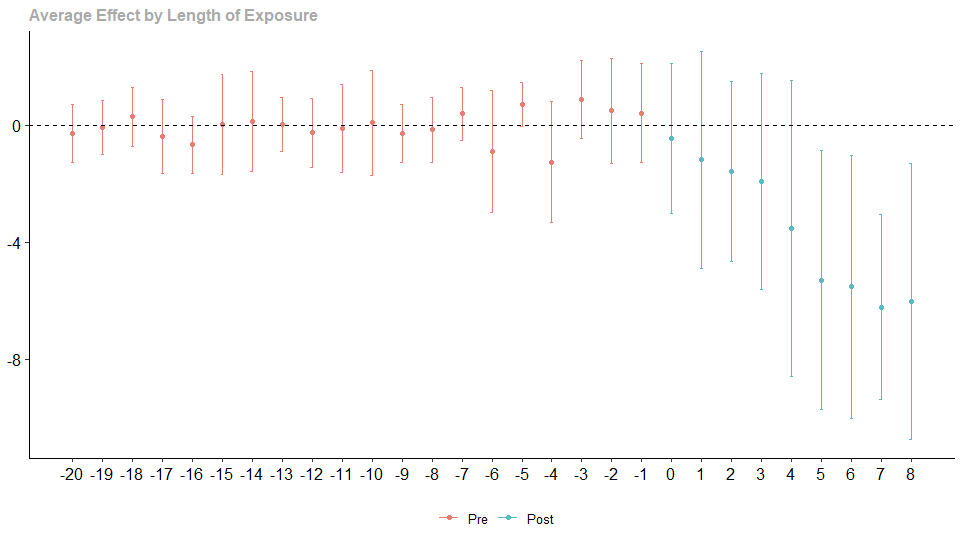
\includegraphics[width=.85\textwidth]{sc_graph.png}
    \end{center}
    \caption{ATT of treatment year on opioid death rate per 100k}
    \label{fig:graph}
\end{figure}

% Table created by stargazer v.5.2.2 by Marek Hlavac, Harvard University. E-mail: hlavac at fas.harvard.edu
% Date and time: Fri, May 06, 2022 - 4:31:24 PM
\begin{table}[!htbp] \centering 
  \caption{Table of ATT Based on Time from Treatment Year} 
  \label{} 
\begin{tabular}[t]{r|r|r|r|r}
\hline
Year from Treatment & ATT & Standard Error & Lower Bound & Upper Bound\\
\hline
-20 & -0.27 & 0.37 & -1.00 & 0.46\\
\hline
-19 & -0.07 & 0.34 & -0.75 & 0.62\\
\hline
-18 & 0.29 & 0.37 & -0.44 & 1.03\\
\hline
-17 & -0.37 & 0.47 & -1.30 & 0.55\\
\hline
-16 & -0.66 & 0.36 & -1.39 & 0.06\\
\hline
-15 & 0.02 & 0.63 & -1.23 & 1.27\\
\hline
-14 & 0.13 & 0.64 & -1.13 & 1.40\\
\hline
-13 & 0.03 & 0.34 & -0.64 & 0.70\\
\hline
-12 & -0.25 & 0.44 & -1.12 & 0.61\\
\hline
-11 & -0.12 & 0.56 & -1.22 & 0.99\\
\hline
-10 & 0.09 & 0.66 & -1.22 & 1.41\\
\hline
-9 & -0.28 & 0.37 & -1.00 & 0.45\\
\hline
-8 & -0.15 & 0.41 & -0.96 & 0.65\\
\hline
-7 & 0.40 & 0.33 & -0.26 & 1.06\\
\hline
-6 & -0.89 & 0.77 & -2.42 & 0.63\\
\hline
-5 & 0.71 & 0.28 & 0.16 & 1.27\\
\hline
-4 & -1.26 & 0.77 & -2.78 & 0.26\\
\hline
-3 & 0.89 & 0.50 & -0.09 & 1.87\\
\hline
-2 & 0.51 & 0.66 & -0.81 & 1.82\\
\hline
-1 & 0.41 & 0.63 & -0.82 & 1.65\\
\hline
0 & -0.43 & 0.95 & -2.31 & 1.45\\
\hline
1 & -1.18 & 1.37 & -3.90 & 1.54\\
\hline
2 & -1.58 & 1.14 & -3.83 & 0.67\\
\hline
3 & -1.93 & 1.36 & -4.63 & 0.77\\
\hline
4 & -3.53 & 1.87 & -7.23 & 0.17\\
\hline
5 & -5.29 & 1.64 & -8.54 & -2.04\\
\hline
6 & -5.51 & 1.66 & -8.80 & -2.22\\
\hline
7 & -6.21 & 1.17 & -8.53 & -3.89\\
\hline
8 & -6.02 & 1.75 & -9.48 & -2.56\\
\hline
\end{tabular}
\end{table} 


%------------------------------------------------------------------------------------------------

\section*{Discussion}

As we expected, opioid deaths goes down after a state legalizes marijuana. However, this does not happen immediately, but takes 5 years for opioids deaths to have a significant decrease. We believe that this is because marijuana becomes a substitute for opioids. 

Even though we find a causal link between opioid deaths and marijuana legalization, we believe that there are ways we could improve this study and some things to consider further. First, there could be selection bias in the states that legalize marijuana. Some of the first adopters of legalized marijuana policies are more liberal and could have other factors that allow them to have less opioid deaths outside of legalizing marijuana. We also notice that less densely populated states have a lower opioid death rate, so it may be worth adding a control for population density or the region of the country.

Also, it is outside the scope of this study to determine if the fall in opioid deaths in state that legalized marijuana led to a higher death rate in another area. It could be possible that the death rate in something such as motor accidents rose while opioid deaths fell.

%------------------------------------------------------------------------------------------------

\section*{Conclusion}

Marijuana legalization leads to less opioid deaths in states that legalize marijuana. This could have a profound effect on policy, as it can become one way to combat the ongoing opioid epidemic. If more states were to adopt marijuana legalization, we may see the opioid crisis begin to slow or even decline. 


%----------------------------------------------------------------------------------------

\end{document}
